% Chapter Backgrpund

\chapter{Background Estimation} \label{chap:4}
In this channel whose final state is four b-flavor jets, main background contribution comes from multi-jet events.
The background estimation in the study combines two methods used in 2015 research: alphabet and bump hunt into alphabet assisted bump hunt\citep{CMS-PAS-B2G-16-008}.
 

\section{Bump Hunt}
The concept of searches for heavy resonance can be seen directly as finding a bump on the top of the smooth background, which is shown in figure 4.1. The fitted target is the mass spectrum of heavy resonances. The prababilty density functions used in fitting are level-exponential function for data and Gaussian for signal.
\begin{figure}[t]
  \centering
  \begin{tabular}{c}
    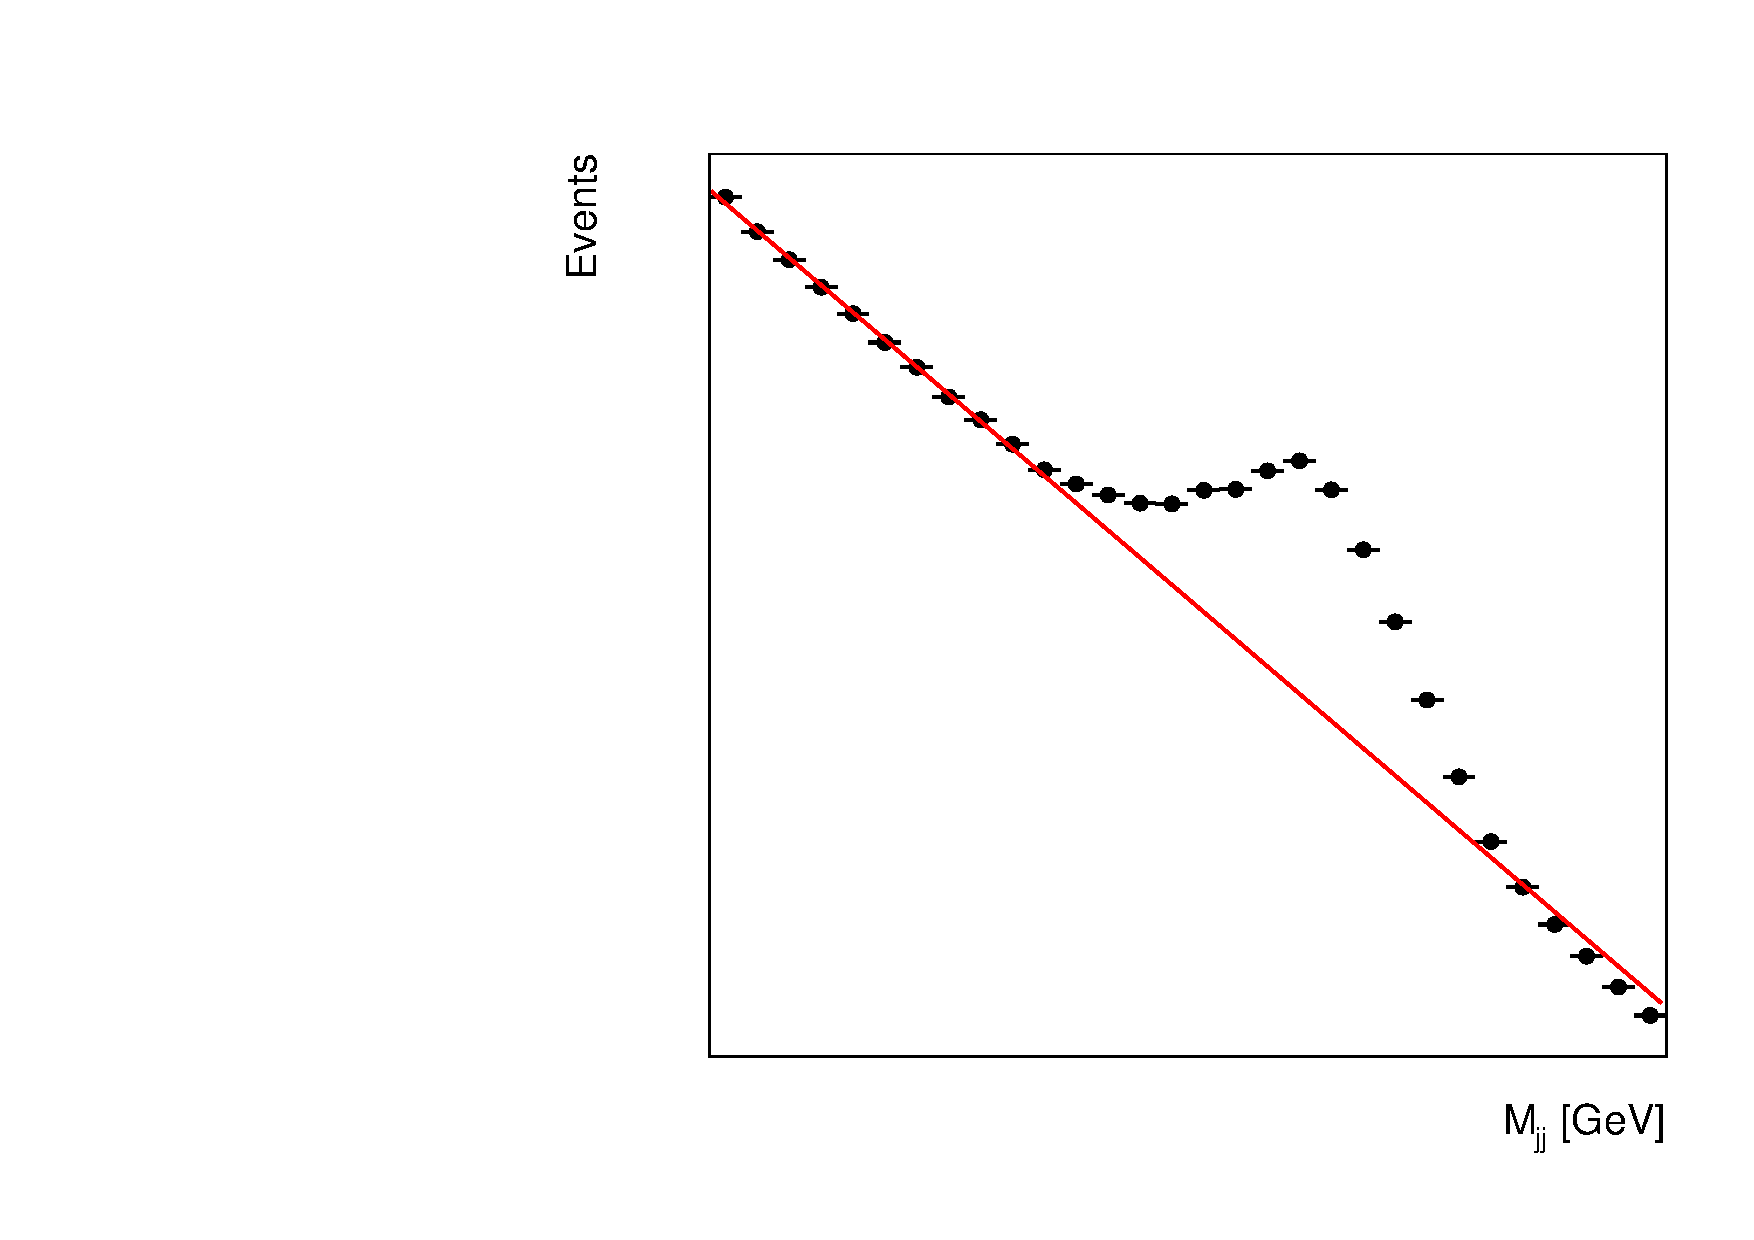
\includegraphics[width=0.5\textwidth]{Figures/cart.pdf} 
   
  \end{tabular}
  \caption{The cartoon of a bump on the background.}
  \label{fig:hvt_brs}
\end{figure}

\section{Alphabet}
Alphabet method evolved from ABCD method which assumes the background is homogenously distributed on the two-dimension histogram. The histogram is sepearted into signal region and sideband region. The background in signal region can be extrapolated from sideband region. For example, if we see the figure 4.2, the number of events in signal region can get by:
\begin{equation} \label{eq1}
\centering
\begin{split}
\frac{N_{signal}}{N_{anti-tag}} = \frac{N_{side band B}}{N_{side band A}} = \frac{N_{side band D}}{N_{side band C}}, \\
N_{signal} = \frac{N_{side band B} \times N_{anti-tag}}{N_{side band A}} = \frac{N_{side band D} \times N_{anti-tag}}{N_{side band C}} \\
= N_{anti-tag} \times R_{p/f}, \\
\end{split}
\end{equation}
where N is the number of events located in the region of square shape. The ratio $\frac{N_{signal}}{N_{anti-tag}}$ is referred as $R_{p/f}$ in the section. If the $R_{p/f}$ has dependence on the mass of the leading AK8 jet, one should use Alphabet method instead of ABCD method, as figure 4.3 and 4.4 show. Alphabet method gives $R_{p/f}$ a dependence on the mass of the leading AK8 jet:
\begin{equation} \label{eq2}
\begin{split}
N_{signal} = N_{anti-tag} \times R_{p/f} (M_{leading AK8}).
\end{split}
\end{equation}
The $R_{p/f}$ is derived in each bin of the mass of leading AK8 jet in mass side band. All $R_{p/f}$ of each bin is fitted together by a quadratic polynominal fit to interpolate the $R_{p/f}$ in the region of mass of signal. The fit results are shown in figure 4.4. Finally, the predicted background is get from filling anti-tagged events weighted according to the mass of its leading AK8 jet. Figure 4.5 is predicted background in both LL and TT region. 

\begin{figure}[t]
  \centering
  \begin{tabular}{c}
    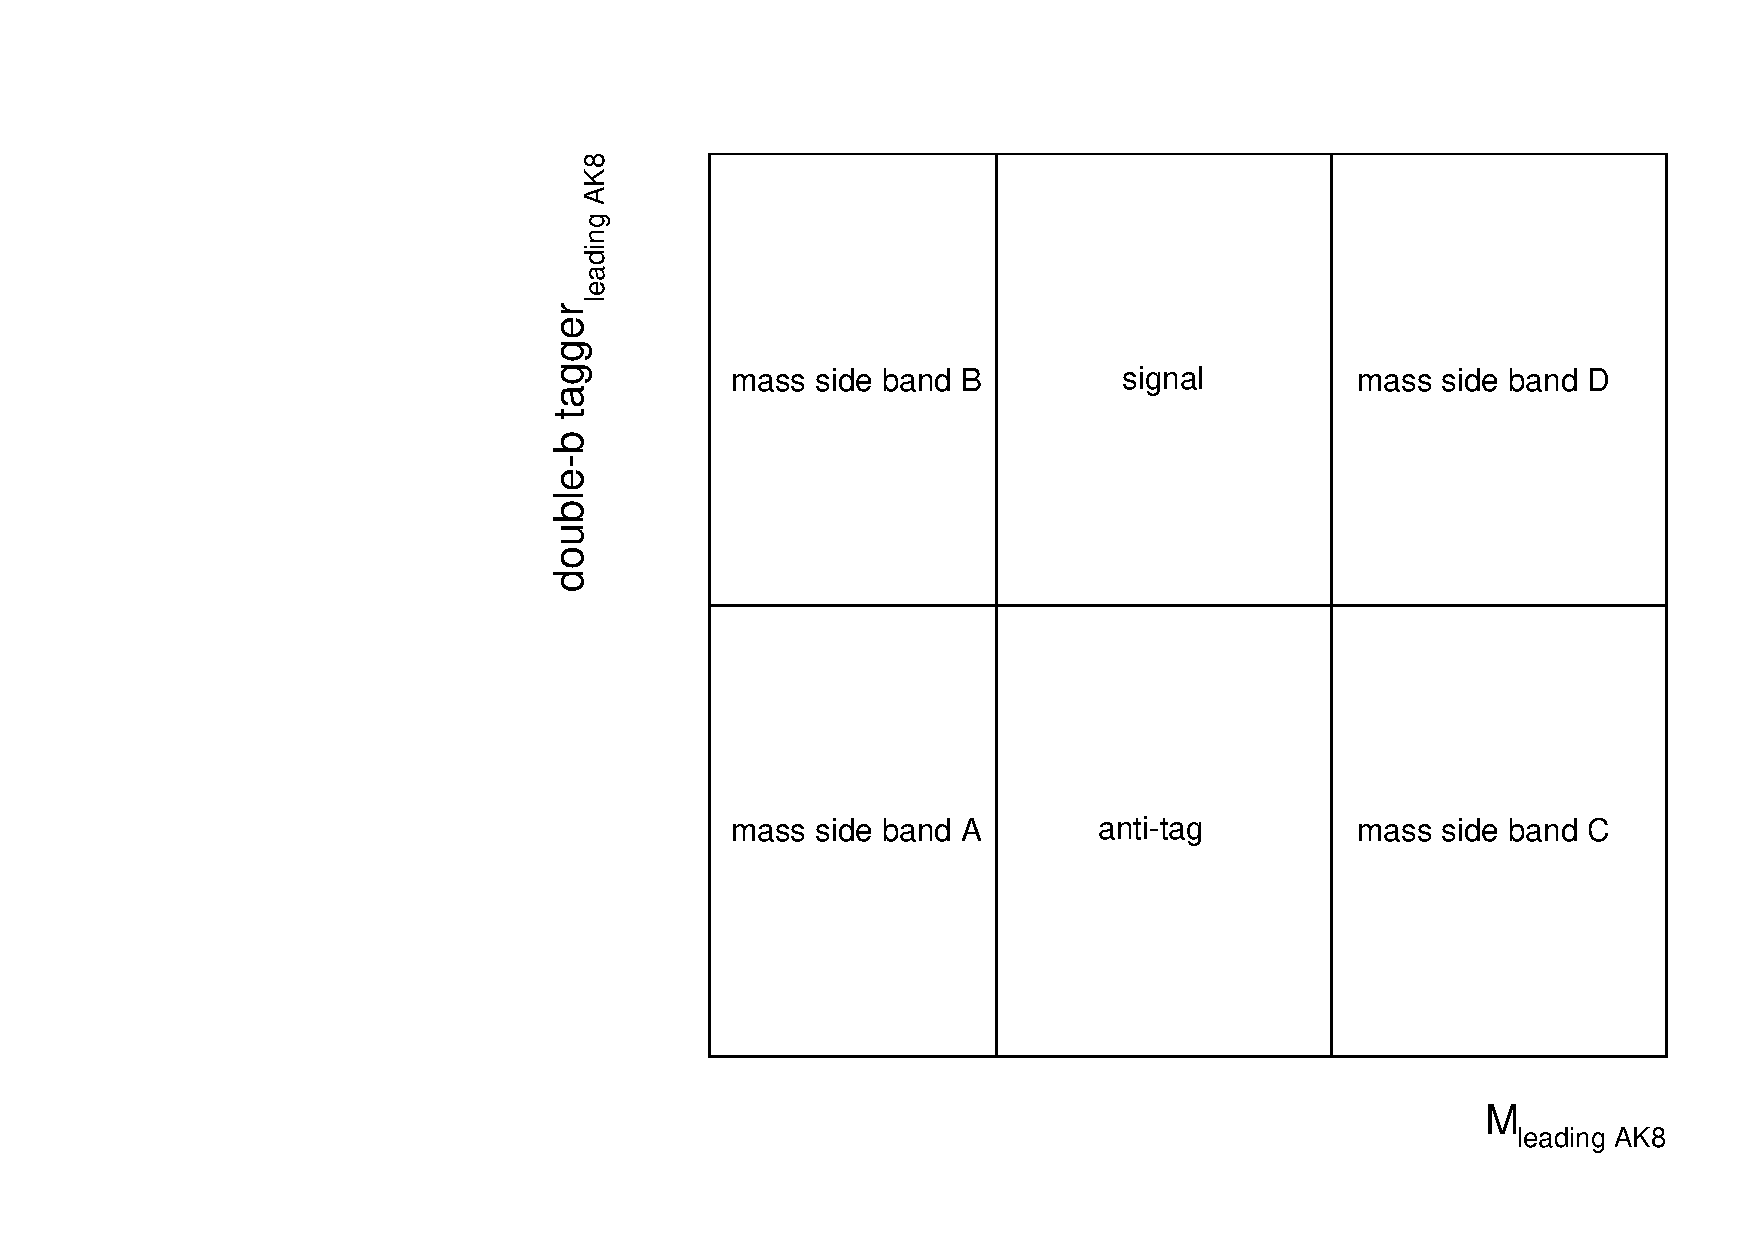
\includegraphics[width=0.5\textwidth]{Figures/cart2.pdf} 
 
  \end{tabular}
  \caption{The cartoon of a two dimensional distribution.}
  \begin{tabular}{cc}
    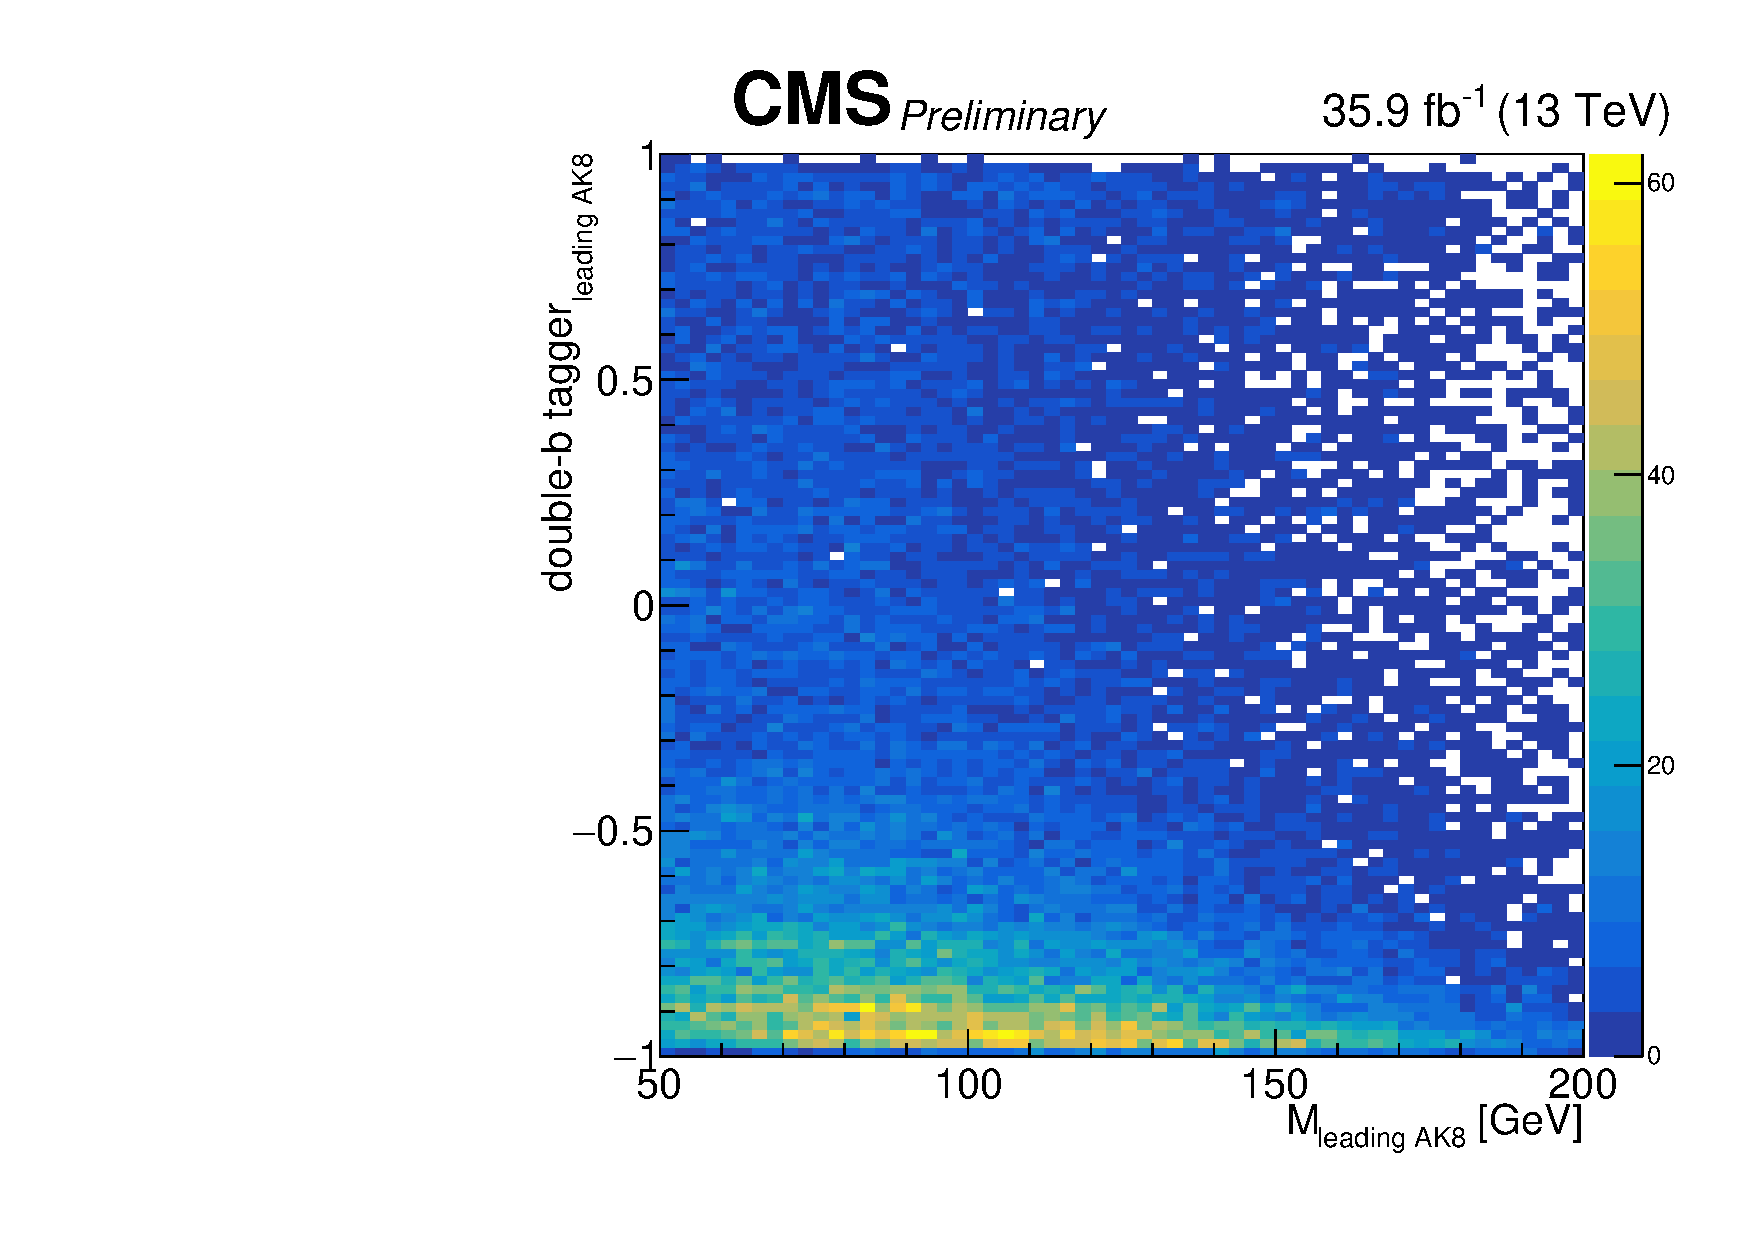
\includegraphics[width=0.5\textwidth]{Figures/al/2d_TT.pdf} &
   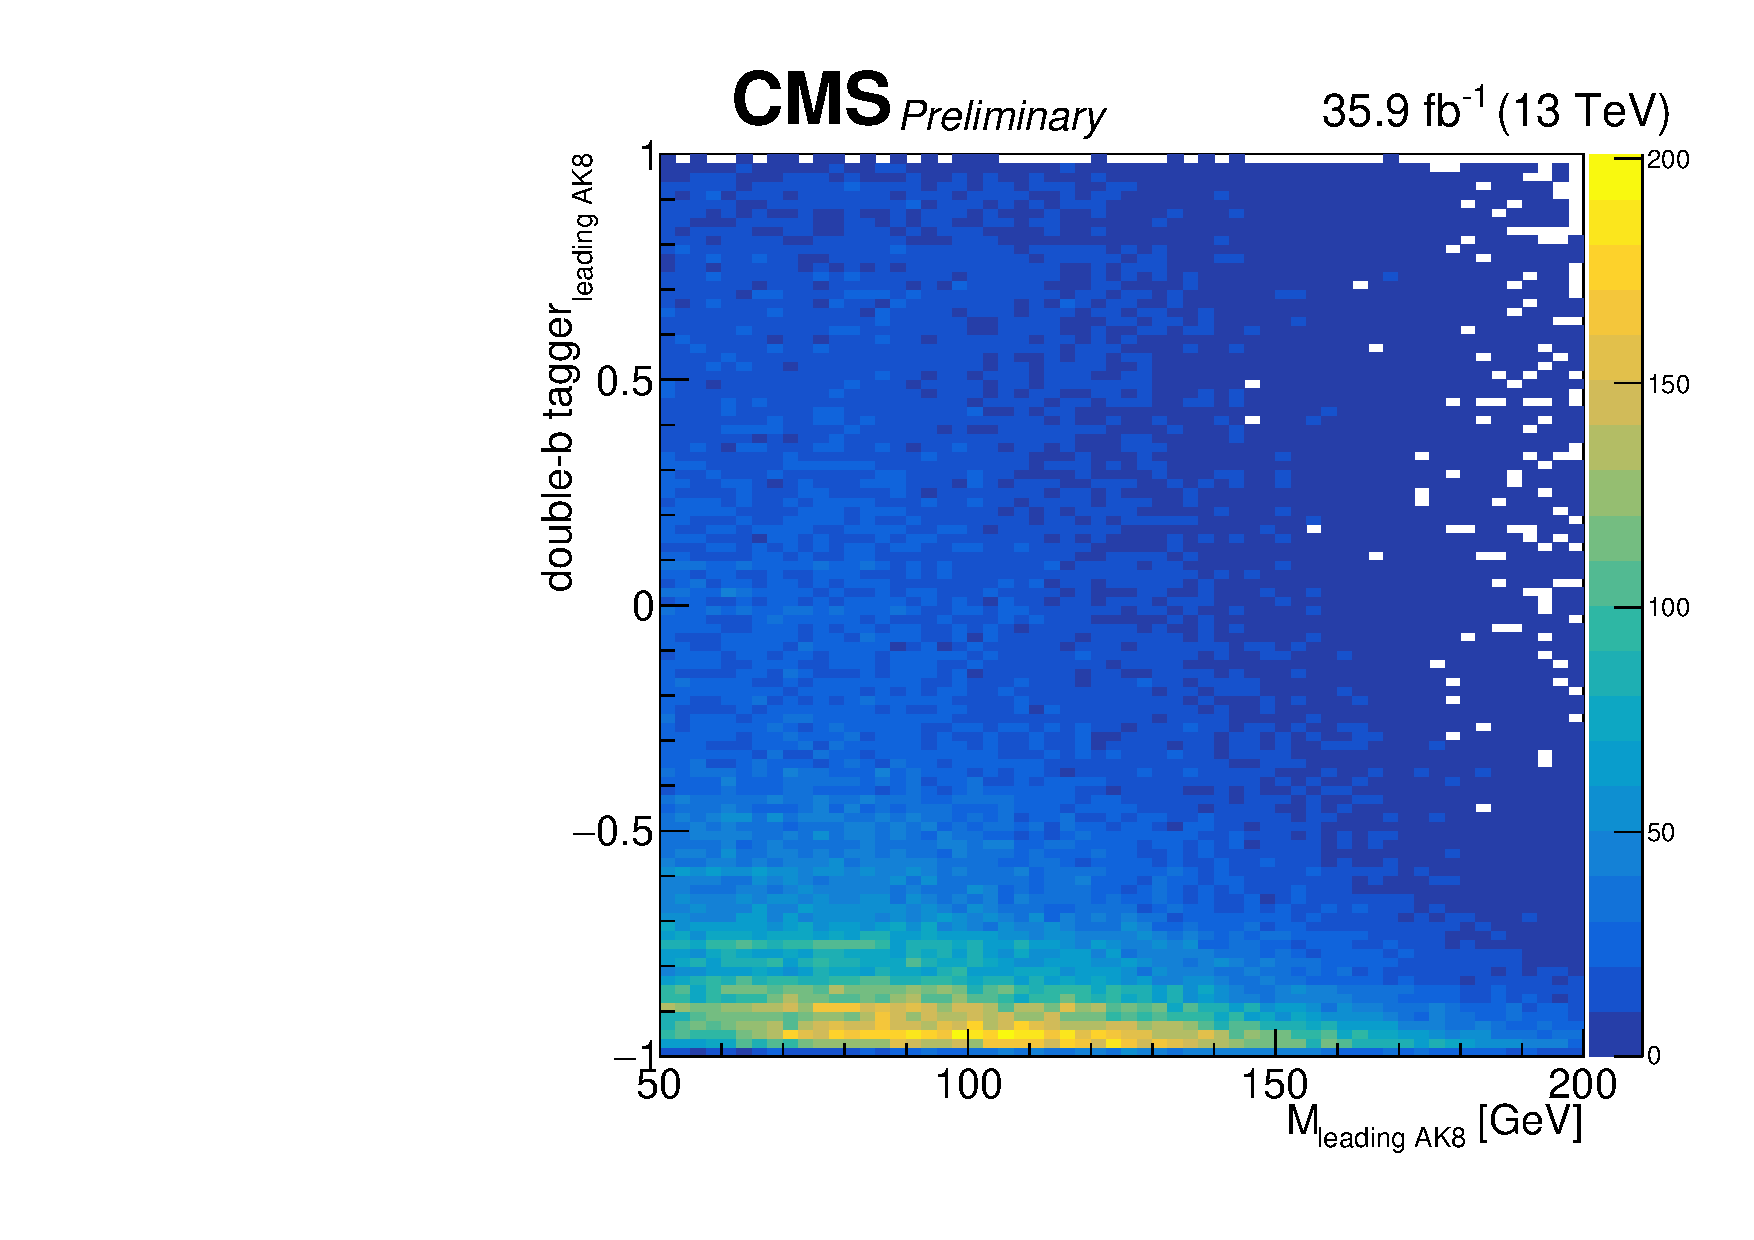
\includegraphics[width=0.5\textwidth]{Figures/al/2d_LL.pdf} 
  \end{tabular}
  \caption{The double-d tagger versus the mass of the leading AK8 jet distribution in TT (left) and LL (right) region.}
\end{figure}



\begin{figure}[t]
  \centering
 \begin{tabular}{cc}
    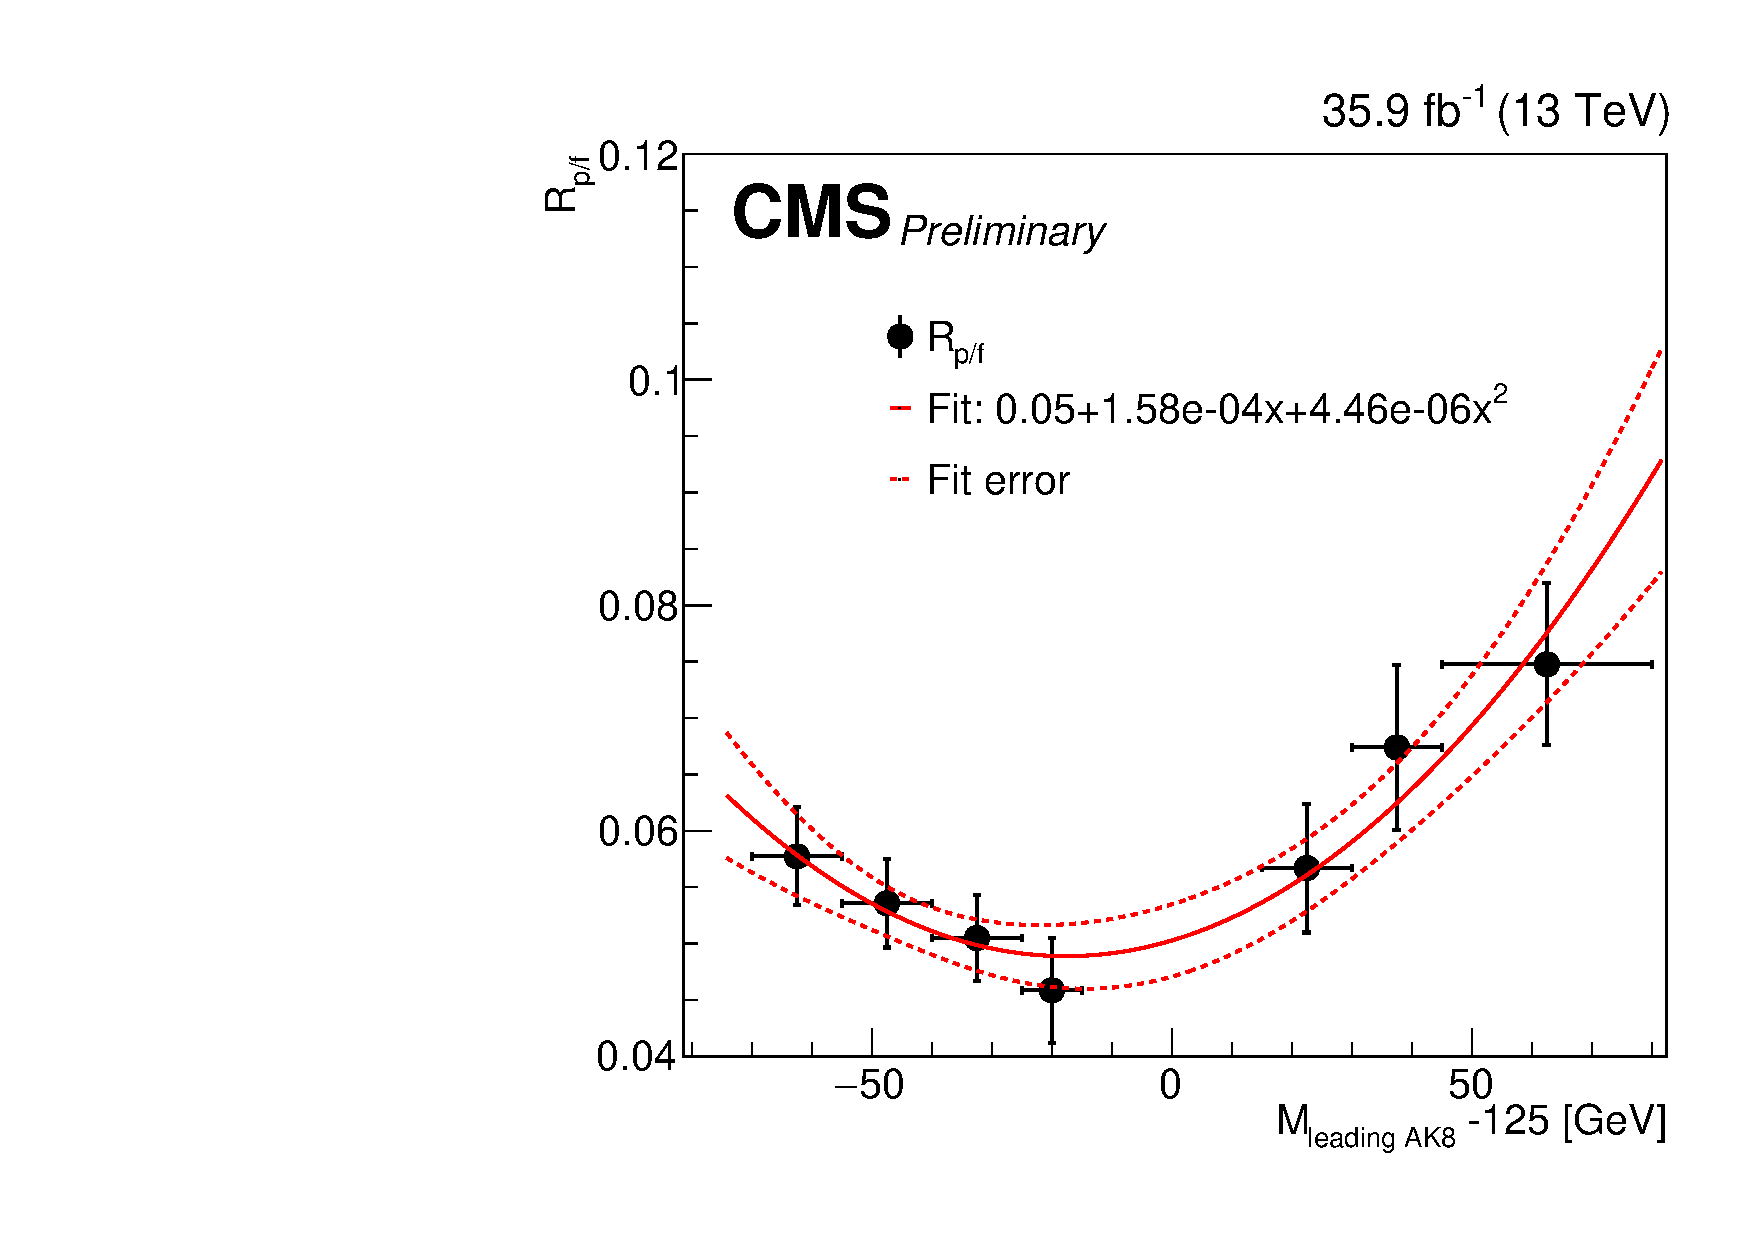
\includegraphics[width=0.5\textwidth]{Figures/al/1d_TT.pdf} &
   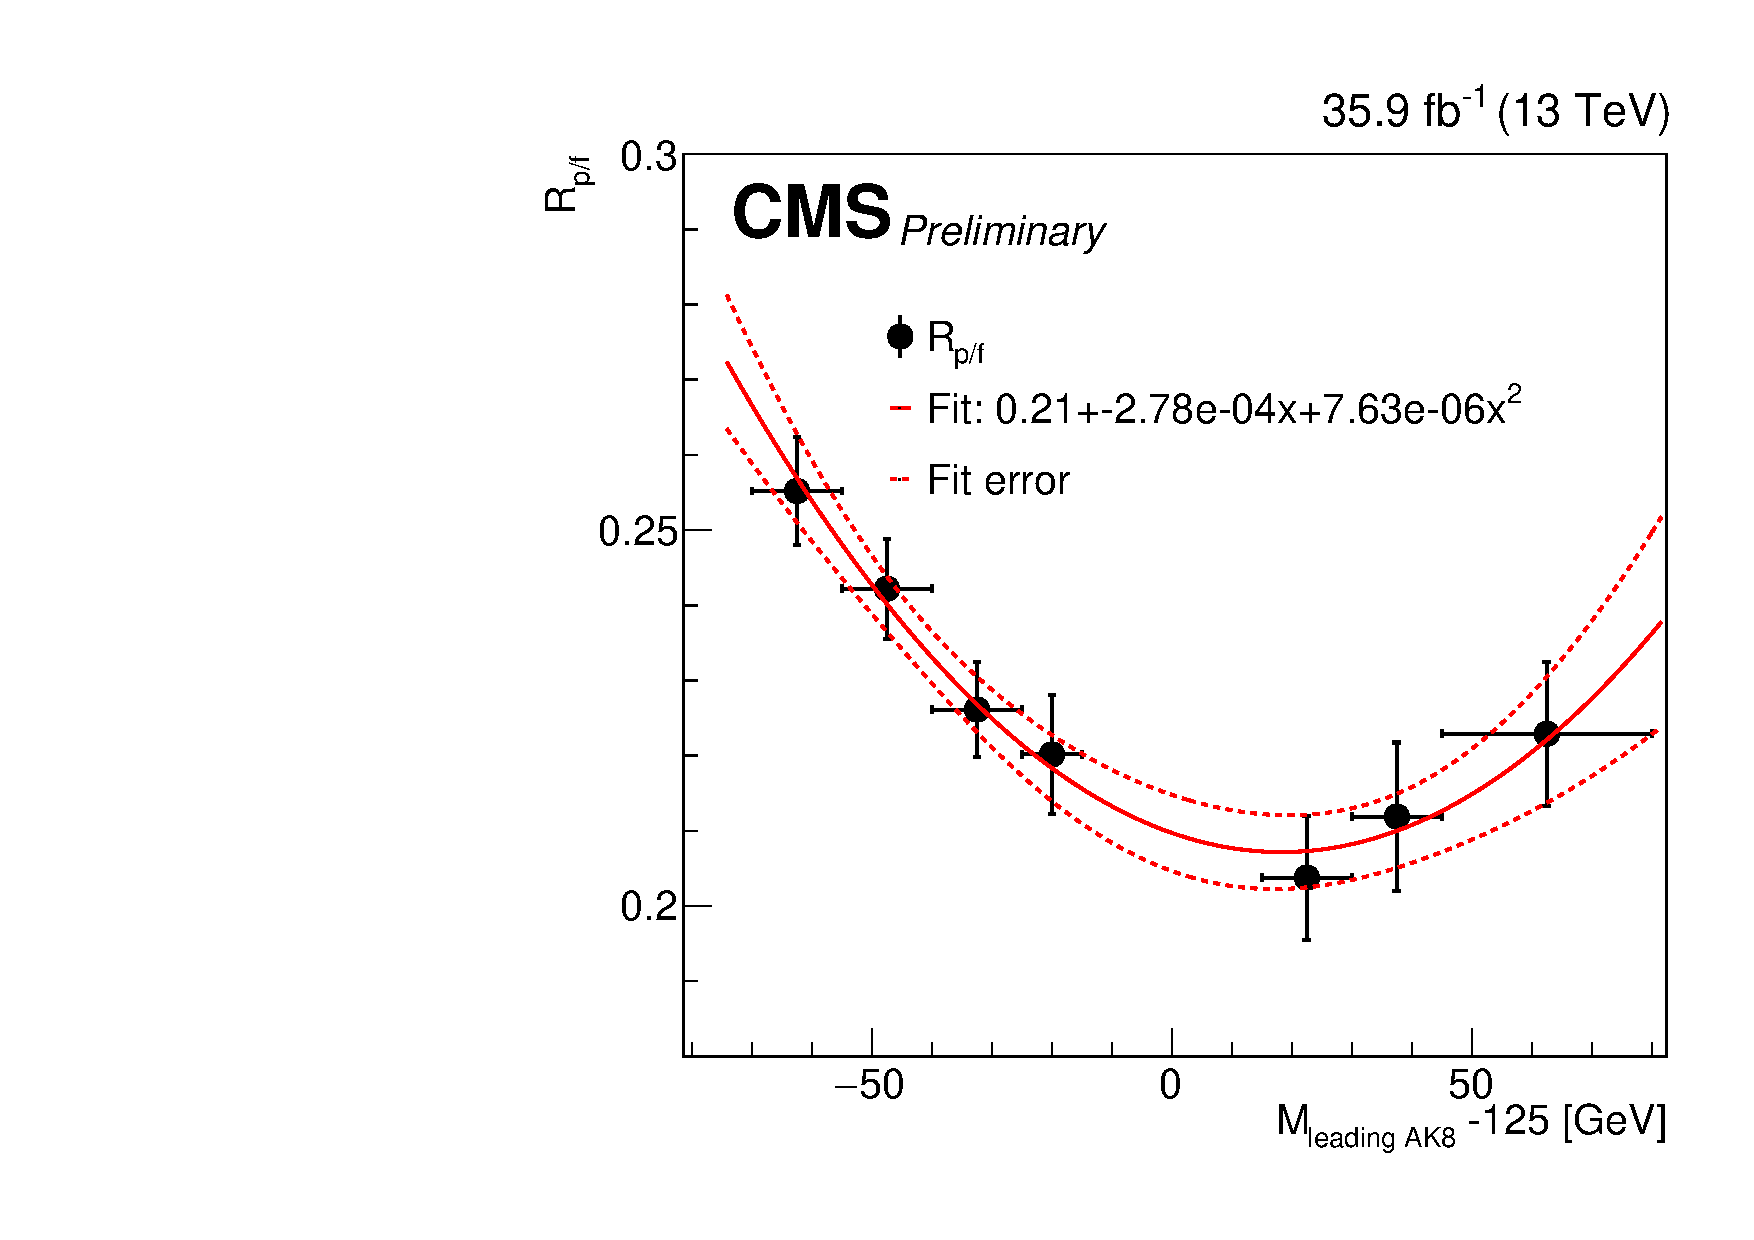
\includegraphics[width=0.5\textwidth]{Figures/al/1d_LL.pdf} 
   
  \end{tabular}
  \caption{The $R_{p/f}$ and its quadratic fit in TT (left) and LL (right) region.}
  \label{fig:hvt_brs}
\end{figure}

\begin{figure}[t]
  \centering
 \begin{tabular}{cc}
    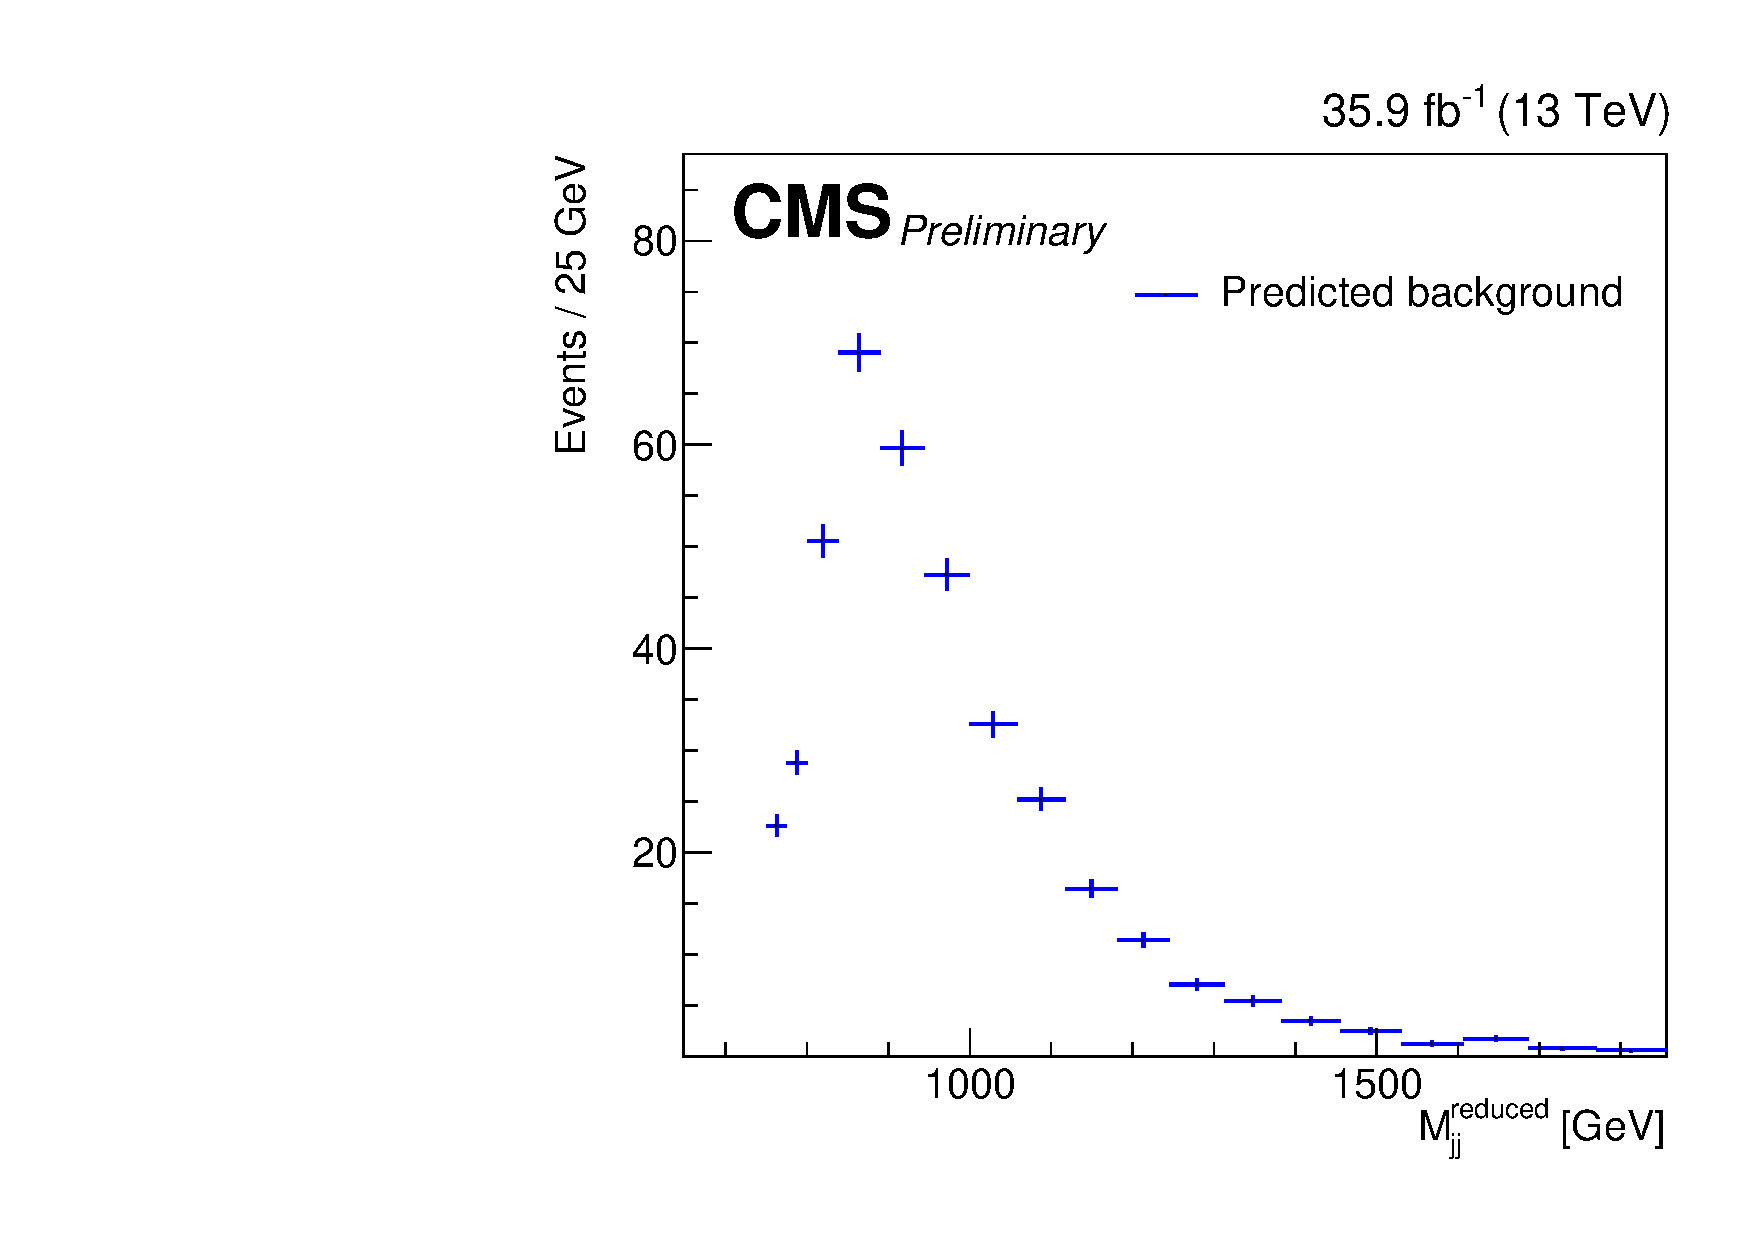
\includegraphics[width=0.5\textwidth]{Figures/al/mjj_TT.pdf} &
   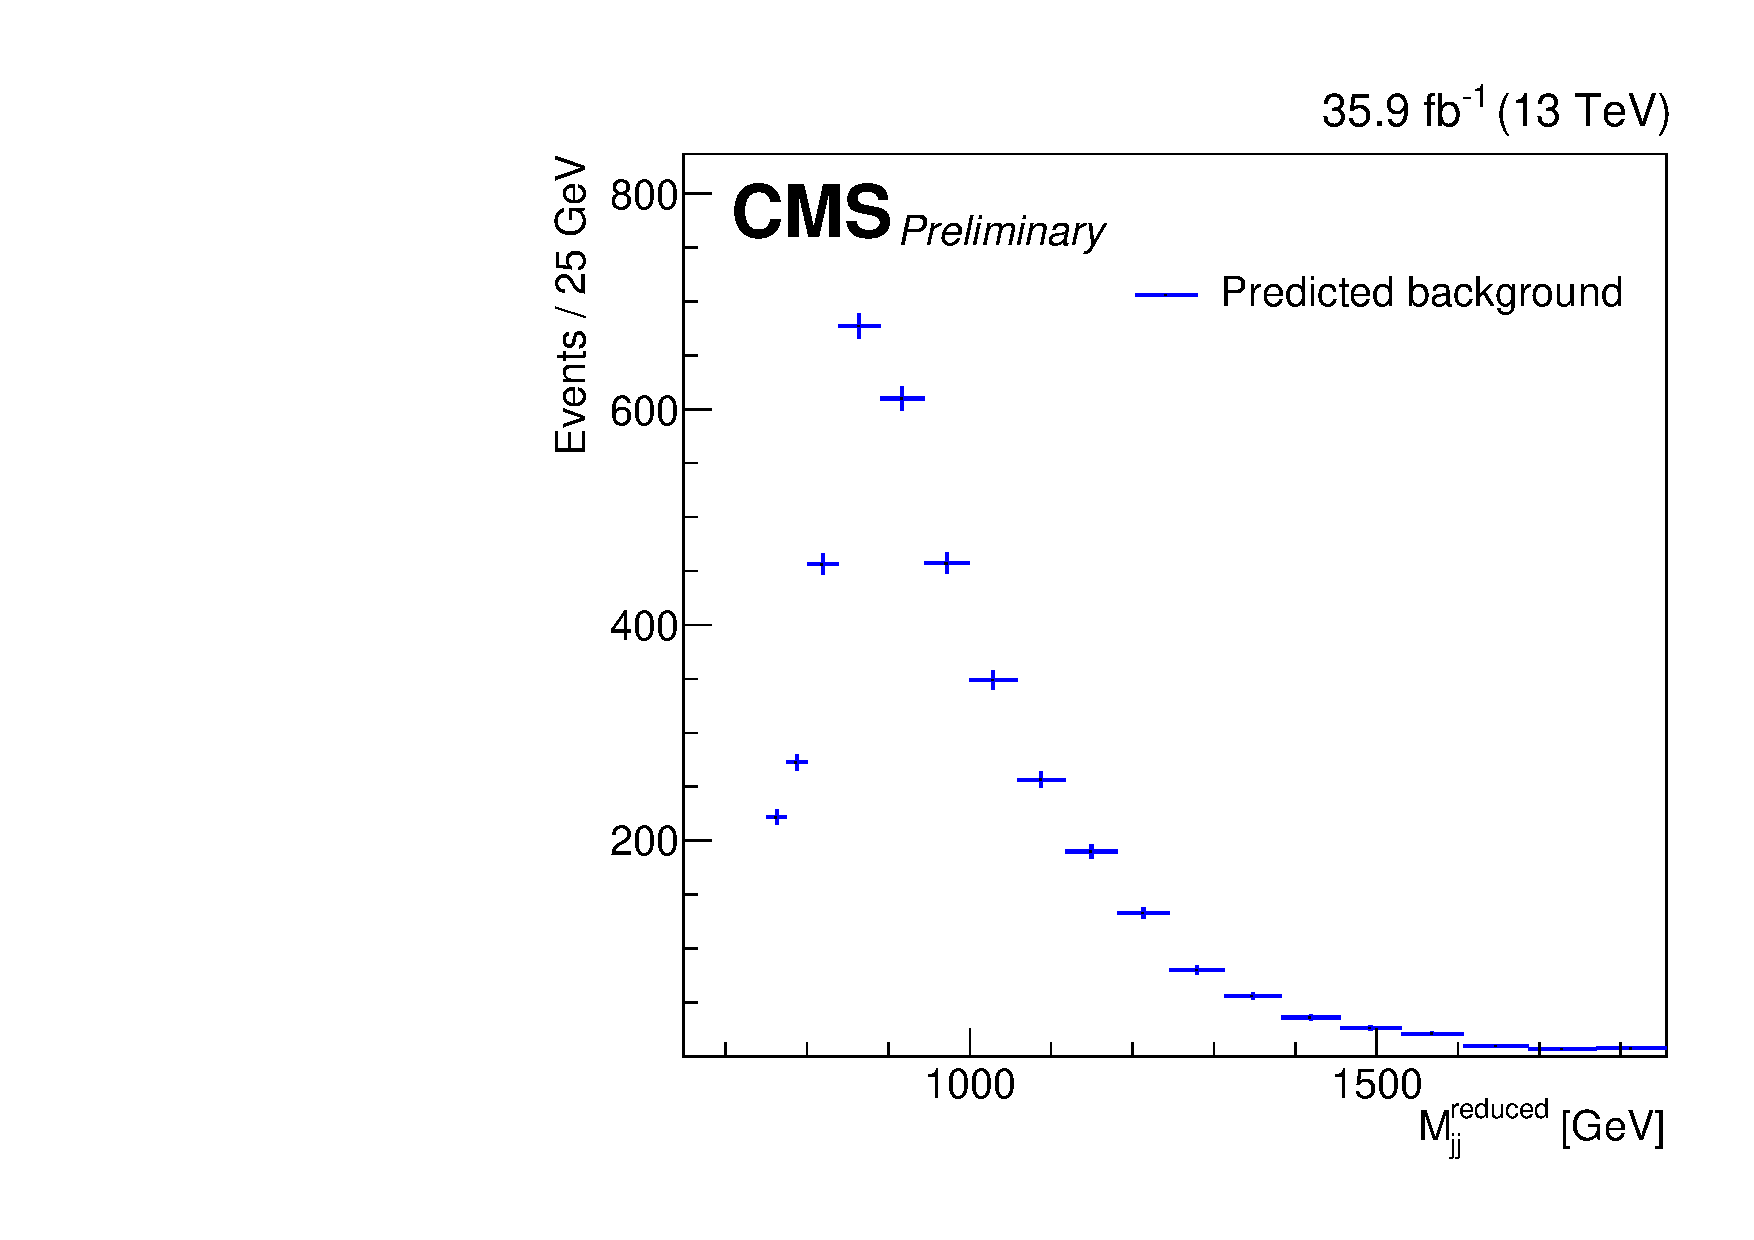
\includegraphics[width=0.5\textwidth]{Figures/al/mjj_LL.pdf} 
   
  \end{tabular}
  \caption{The predicted background from data in TT (left) and LL (right) region.}
  \label{fig:hvt_brs}
\end{figure}

\clearpage
\section{Alphabet Assisted Bump Hunt}
The two background estimation methods, alphabet and bump hunt, use orthogonal information from data.
While bump hunt drives in signal region, alphabet extrapolates from data in side band region. 
Therefore, we can combine two method into alphabet assisted bump hunt. The estimation is inplemented as follow:
\begin{itemize}
\item Define a tagging and anti-tagging region. The double-b tagger working point is used as a discriminator here.
\item Derive the ratio of number of events in tagging region to that of anti-tagging region, which referred below $" R_{p/f} "$.
\item The dependence of $R_{p/f}$ on $M_{jj}$ and that on $M_{Higgs Jet}$ are considered, while the latter is small enough to be ignored. The shape and the numbner of estimated background can be get from:
\begin{equation} \label{eq3}
\begin{split}
Bkg(M_{jj})= R_{p/f}(M_{jj}) \times Anti-tag(M_{jj}), 
\end{split}
\end{equation}
which can be further reduced to 
\begin{equation} \label{eq4}
\begin{split}
R_{p/f}(M_{jj})= 1+(M_{jj} \times lin_{par}) \\
Bkg(M_{jj})= (1+(M_{jj} \times lin_{par})) \times Anti-tag(M_{jj}),
\end{split}
\end{equation}
where Bkg($M_{jj}$) is not get from the p.d.f of Anti-tag, rather it get from fitting to the histogram of reduced mass in signal region directly.
The parameters in the p.d.f of Anti-tag($M_{jj}$) share the same parameters of Bkg($M_{jj}$), and $lin_{par}$ is a parameter of the linear dependence on $M_{jj}$. The initialized p.d.f is referred as pre-fit.
\item  The parameters of the p.d.f. of Bkg($M_{jj}$) are retrained. The p.d.f. of Anti-tag($M_{jj}$) is fitted to the histogram of reduced mass in anti-tagged region. As both p.d.f. share the same parameters, the p.d.f. of Bkg($M_{jj}$) is changed using the value of the parameters of Anti-tag($M_{jj}$) to finish a post-fit procedure. 
\subsection{Signal model}
The signal model is a combination of Guassian and Crystal ball p.d.f. with the same mean. The p.d.f.s fitted to the signal are shown in figure 4.6.  
\begin{figure}[t]
  \centering
 \begin{tabular}{cc}
    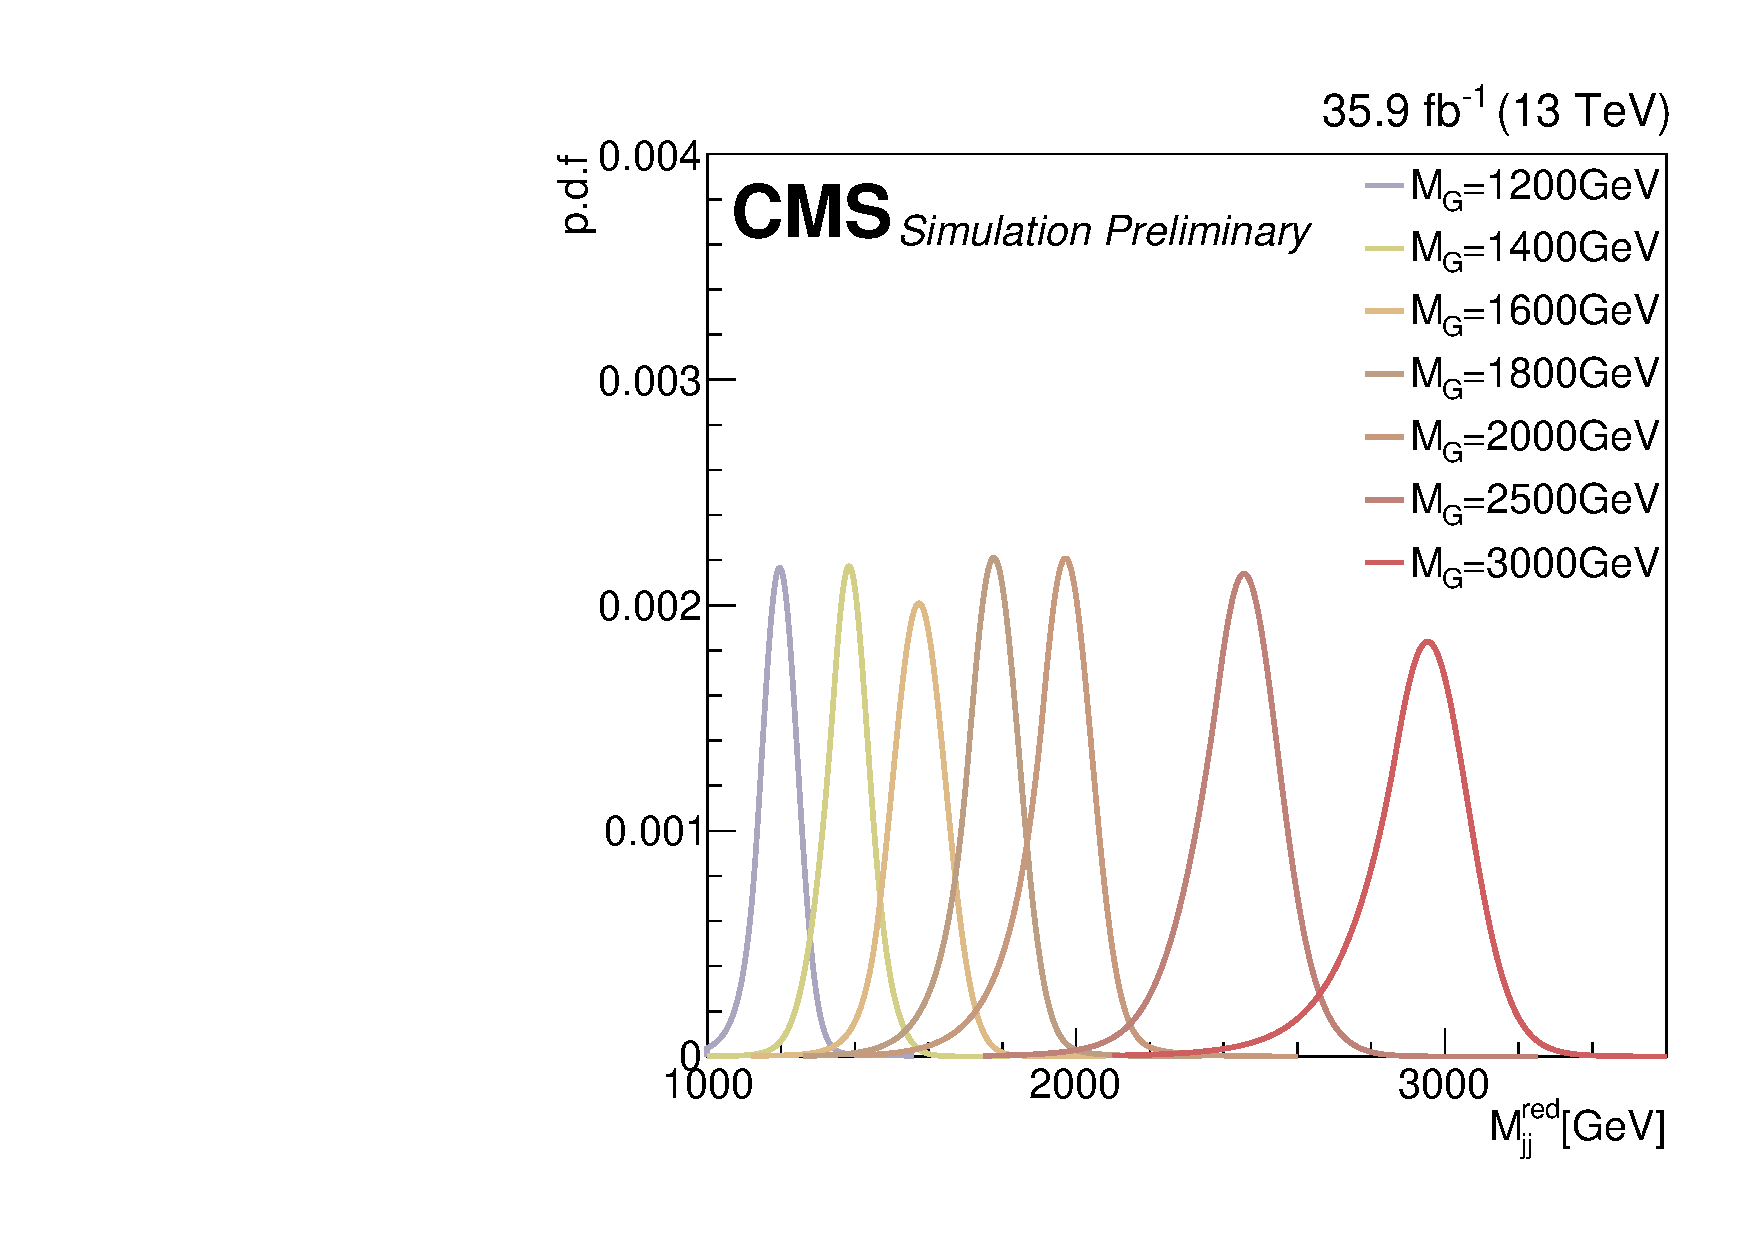
\includegraphics[width=0.5\textwidth]{Figures/sigMod/TT.pdf} &
   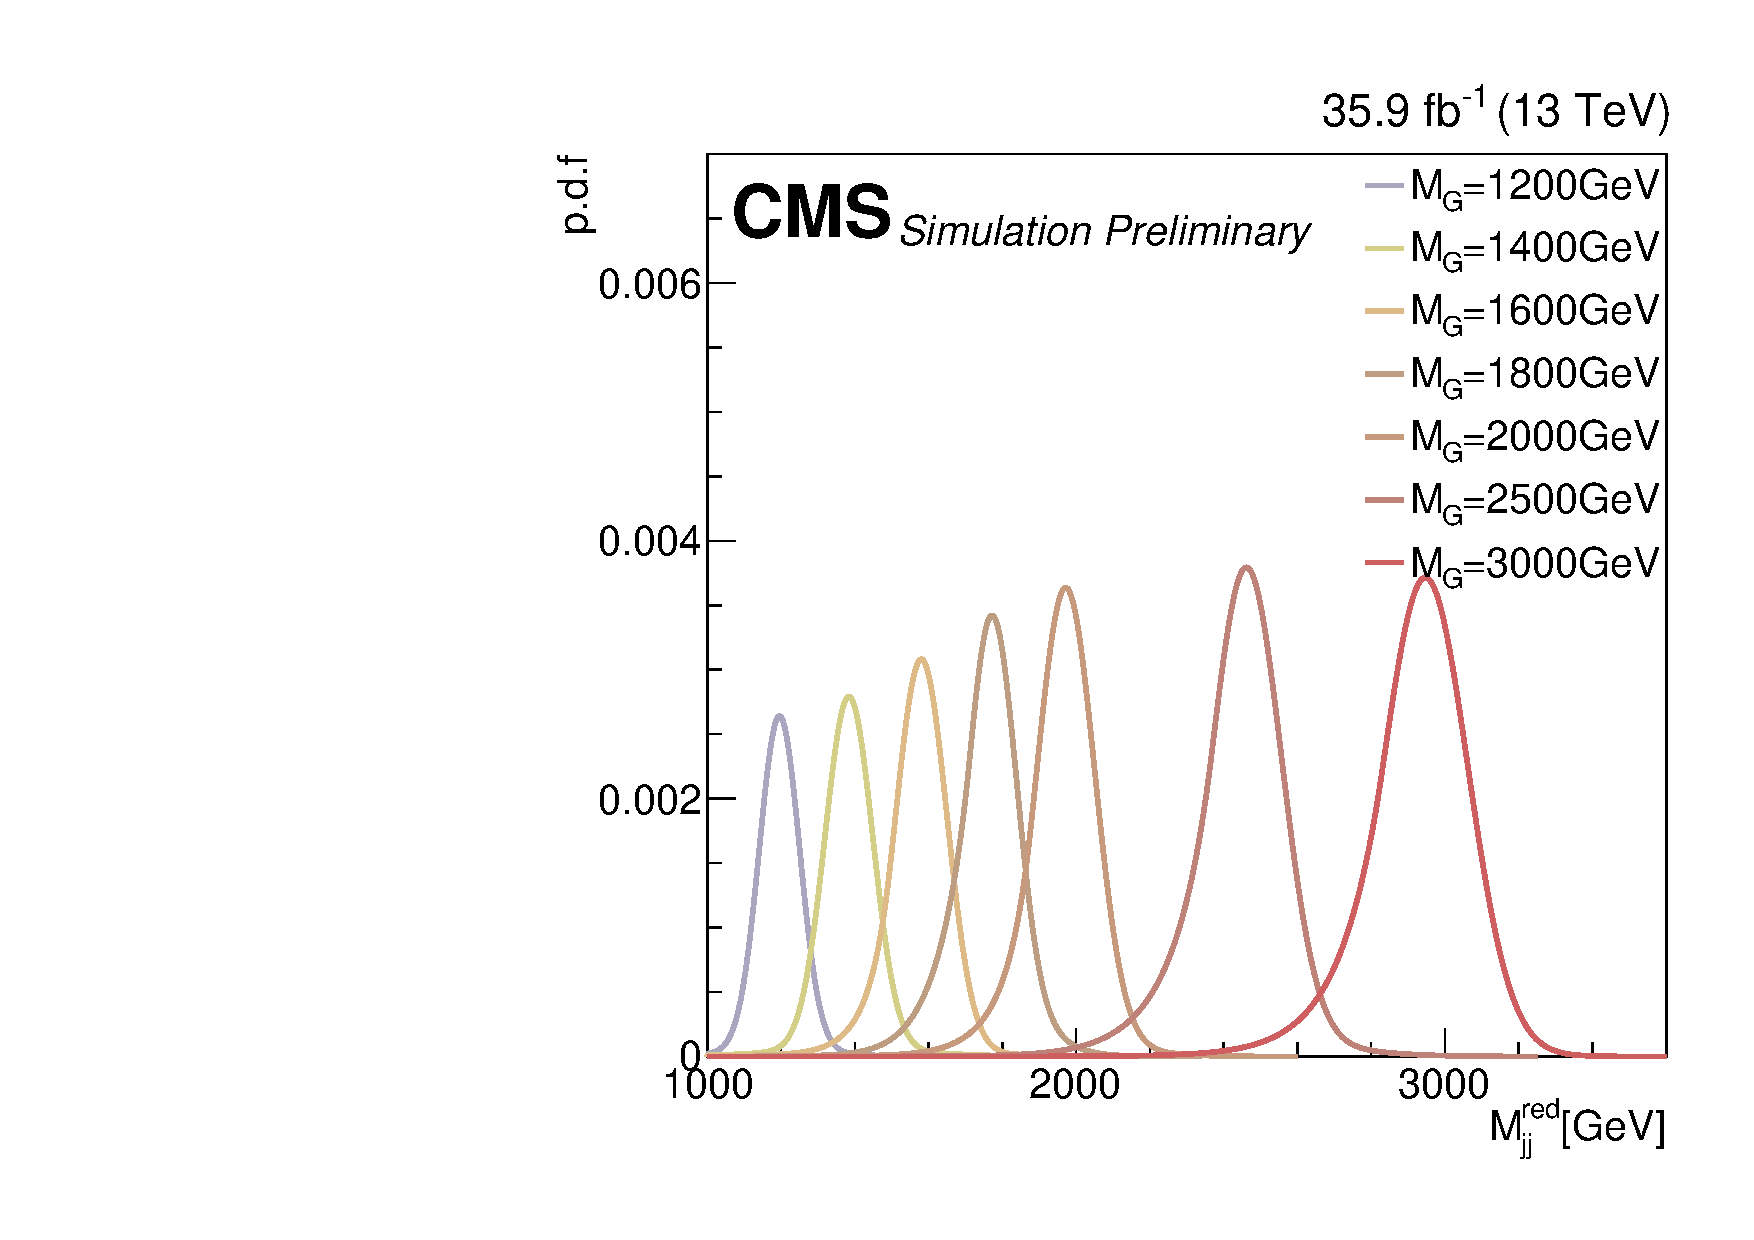
\includegraphics[width=0.5\textwidth]{Figures/sigMod/LL.pdf} \\
  \end{tabular}
  \caption{The p.d.f. of signal model in TT (left) and LL (right) category.The signal of Bulk raviton is used.The p.d.f.s are normalized to integral of all probabilty of one.}
  \label{fig:hvt_brs}
\end{figure}

\subsection{Background model}
The background model is chosen to describe the exponential-decay distribution of the reduced mass. Therefore, levelled expoential p.d.f. is used to fit to the shape. There is little difference between the form of the p.d.f used for signal region and for anti-tagged region. The p.d.f.s after fitted to the histogram in the pre-fit and post-fit procedure are shown in the figure 4.7. % to-do
\begin{equation} \label{eq5}
\begin{split}
Bkg_{sig} = N \times (1 + lin \times M^{red}_{jj})e^{\frac{M^{red}_{jj}\times p1}{1+M^{red}_{jj} \times p1 \times p2}}, \\
Bkg_{anti} = N \times e^{\frac{M^{red}_{jj}\times p1}{1+M^{red}_{jj} \times p1 \times p2}},
\end{split} 
\end{equation}



\begin{figure}[t]
  \centering
 \begin{tabular}{cc}
    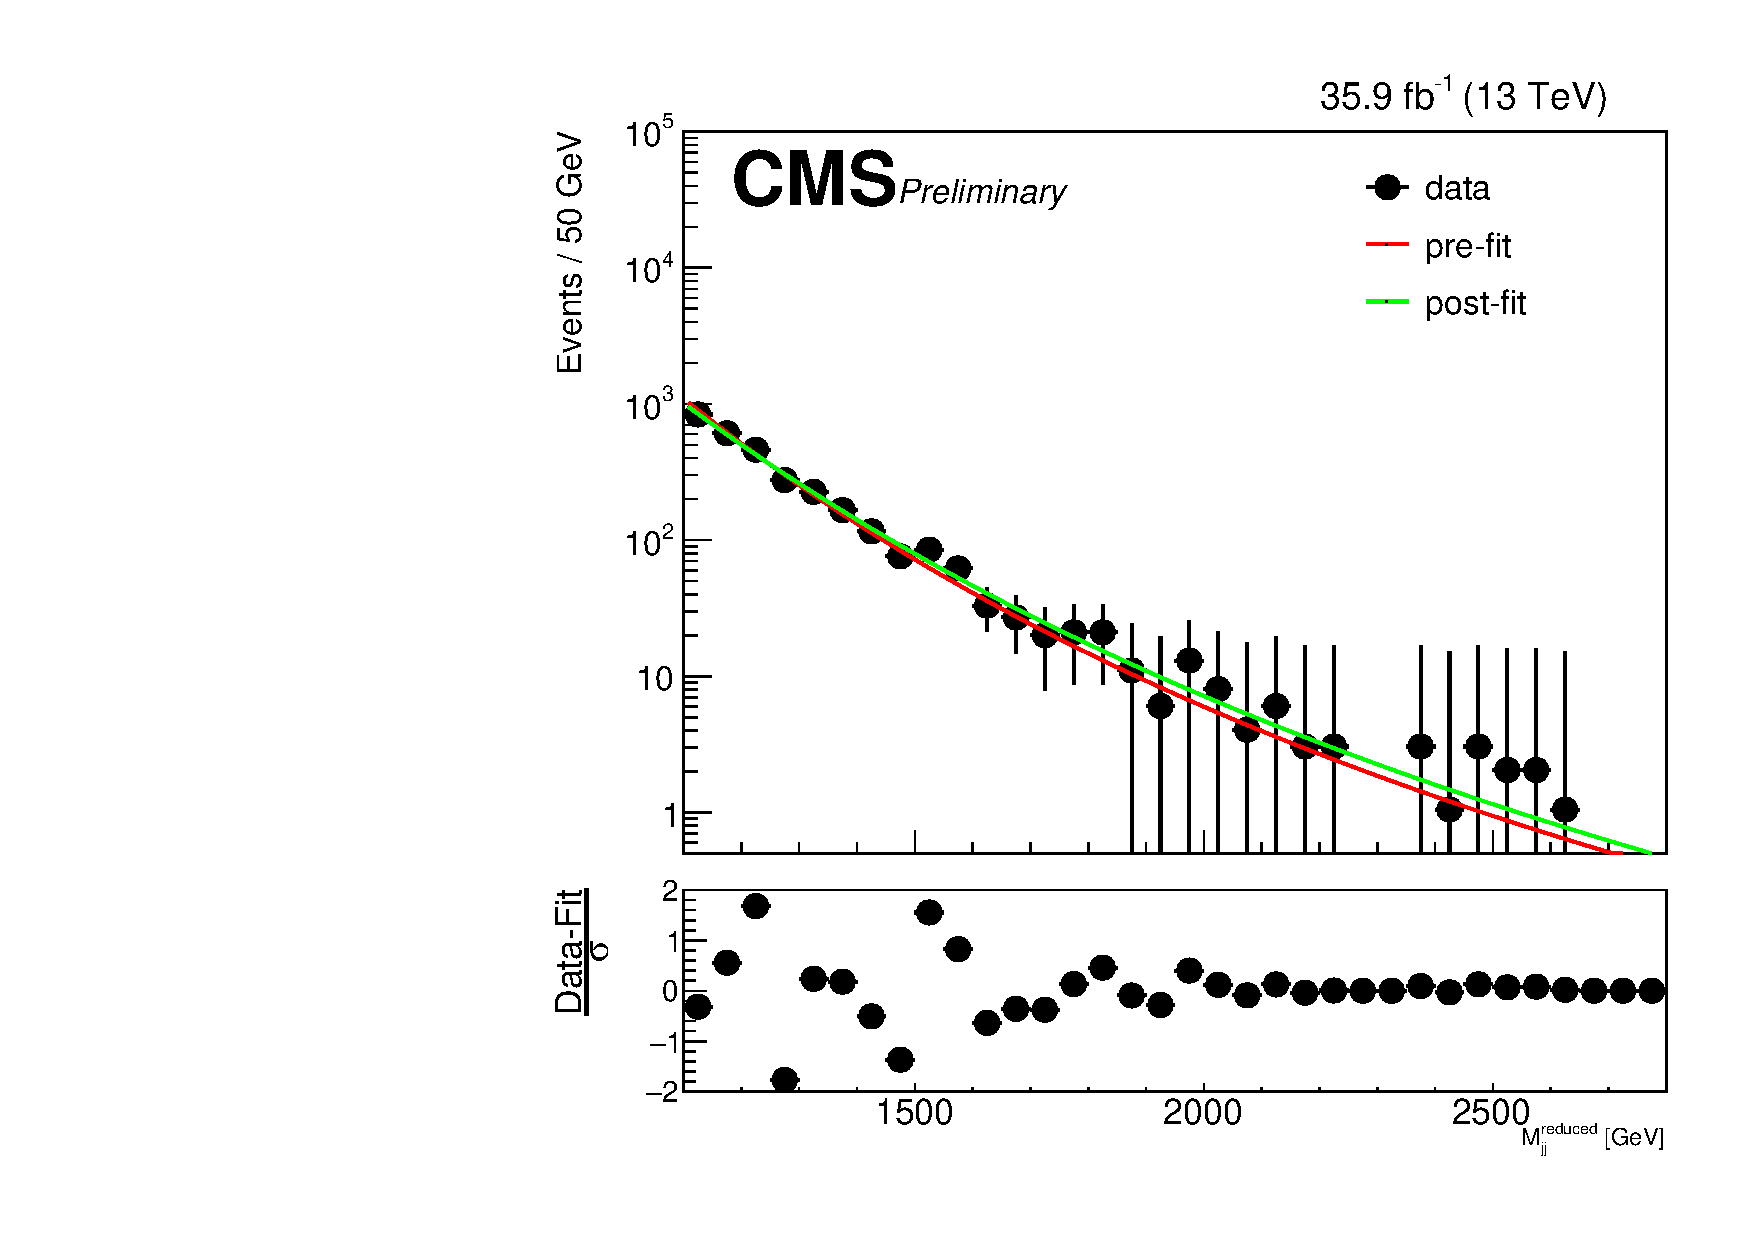
\includegraphics[width=0.5\textwidth]{Figures/aa/anti_LL.pdf} &
   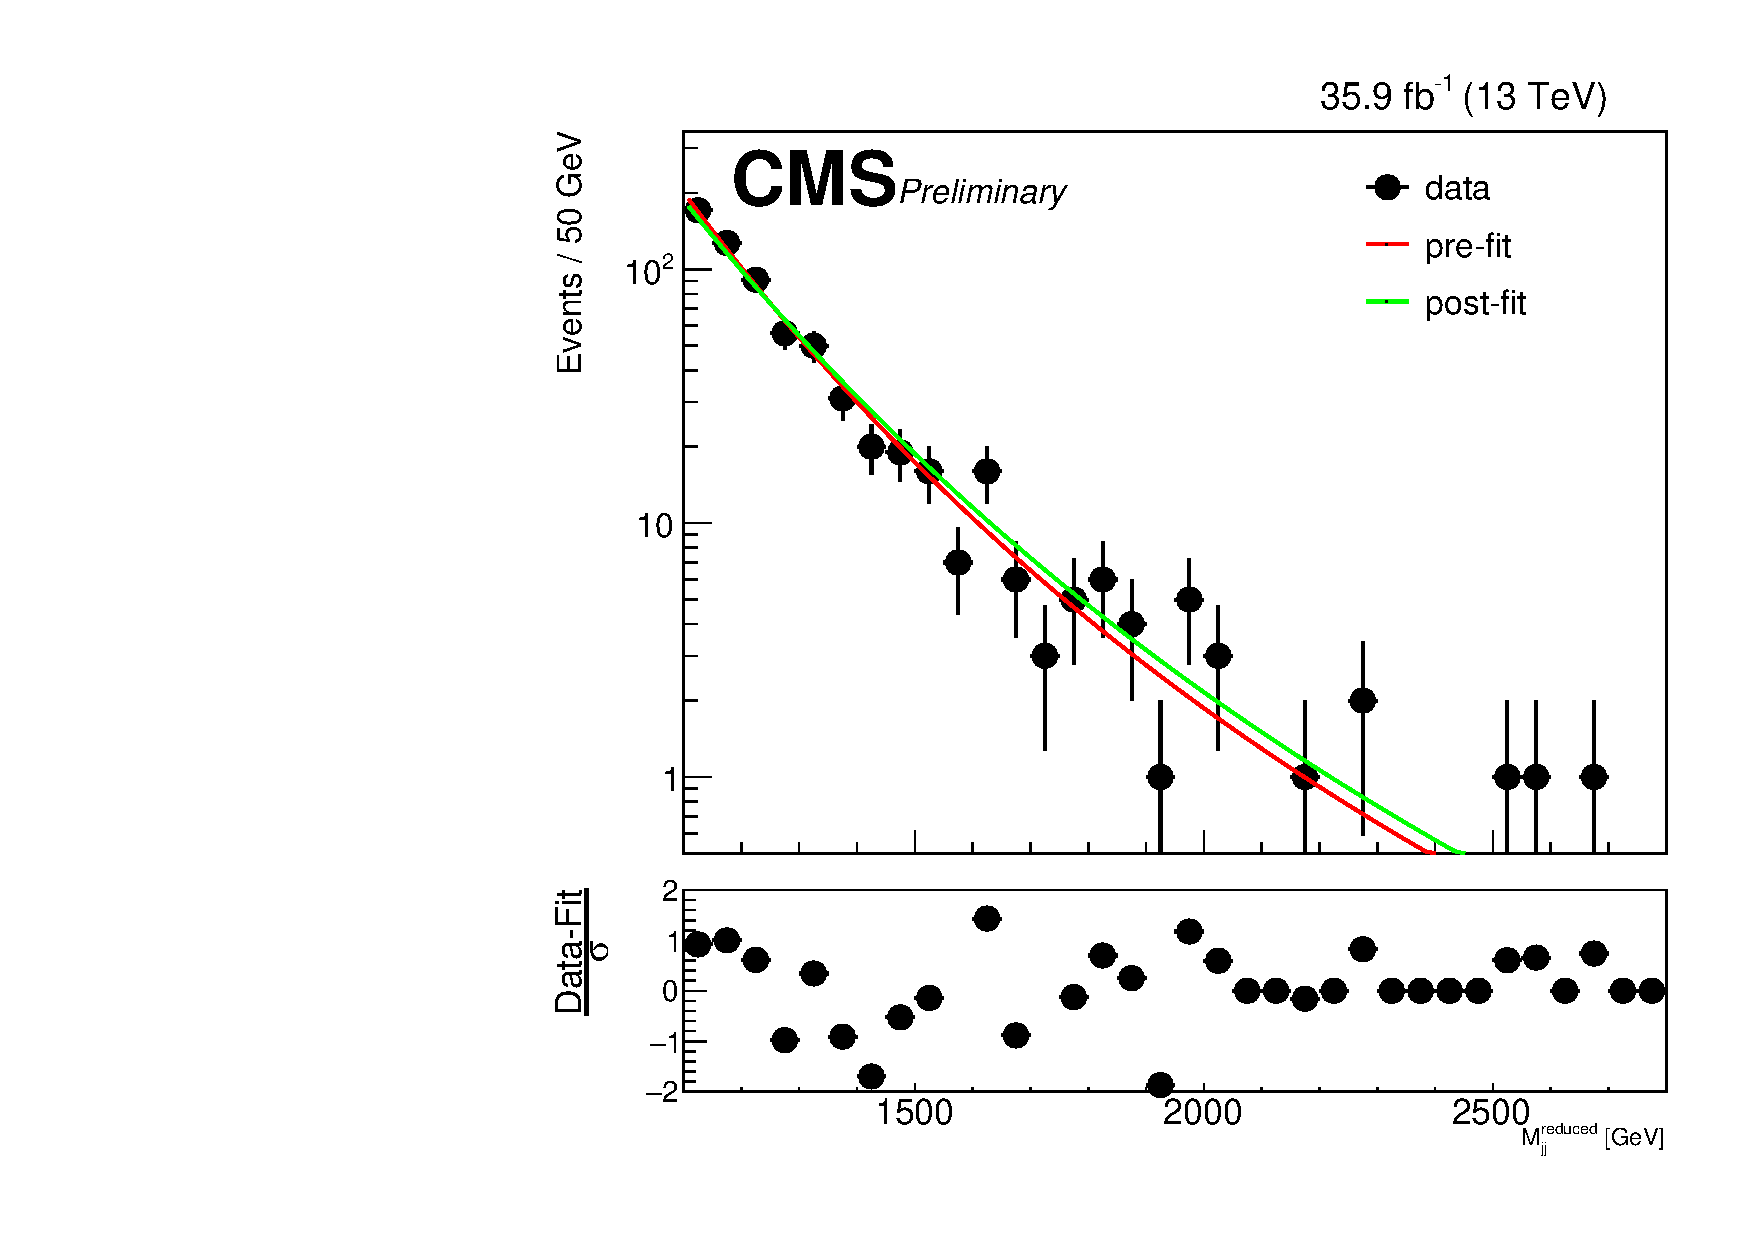
\includegraphics[width=0.5\textwidth]{Figures/aa/data_LL.pdf} \\
   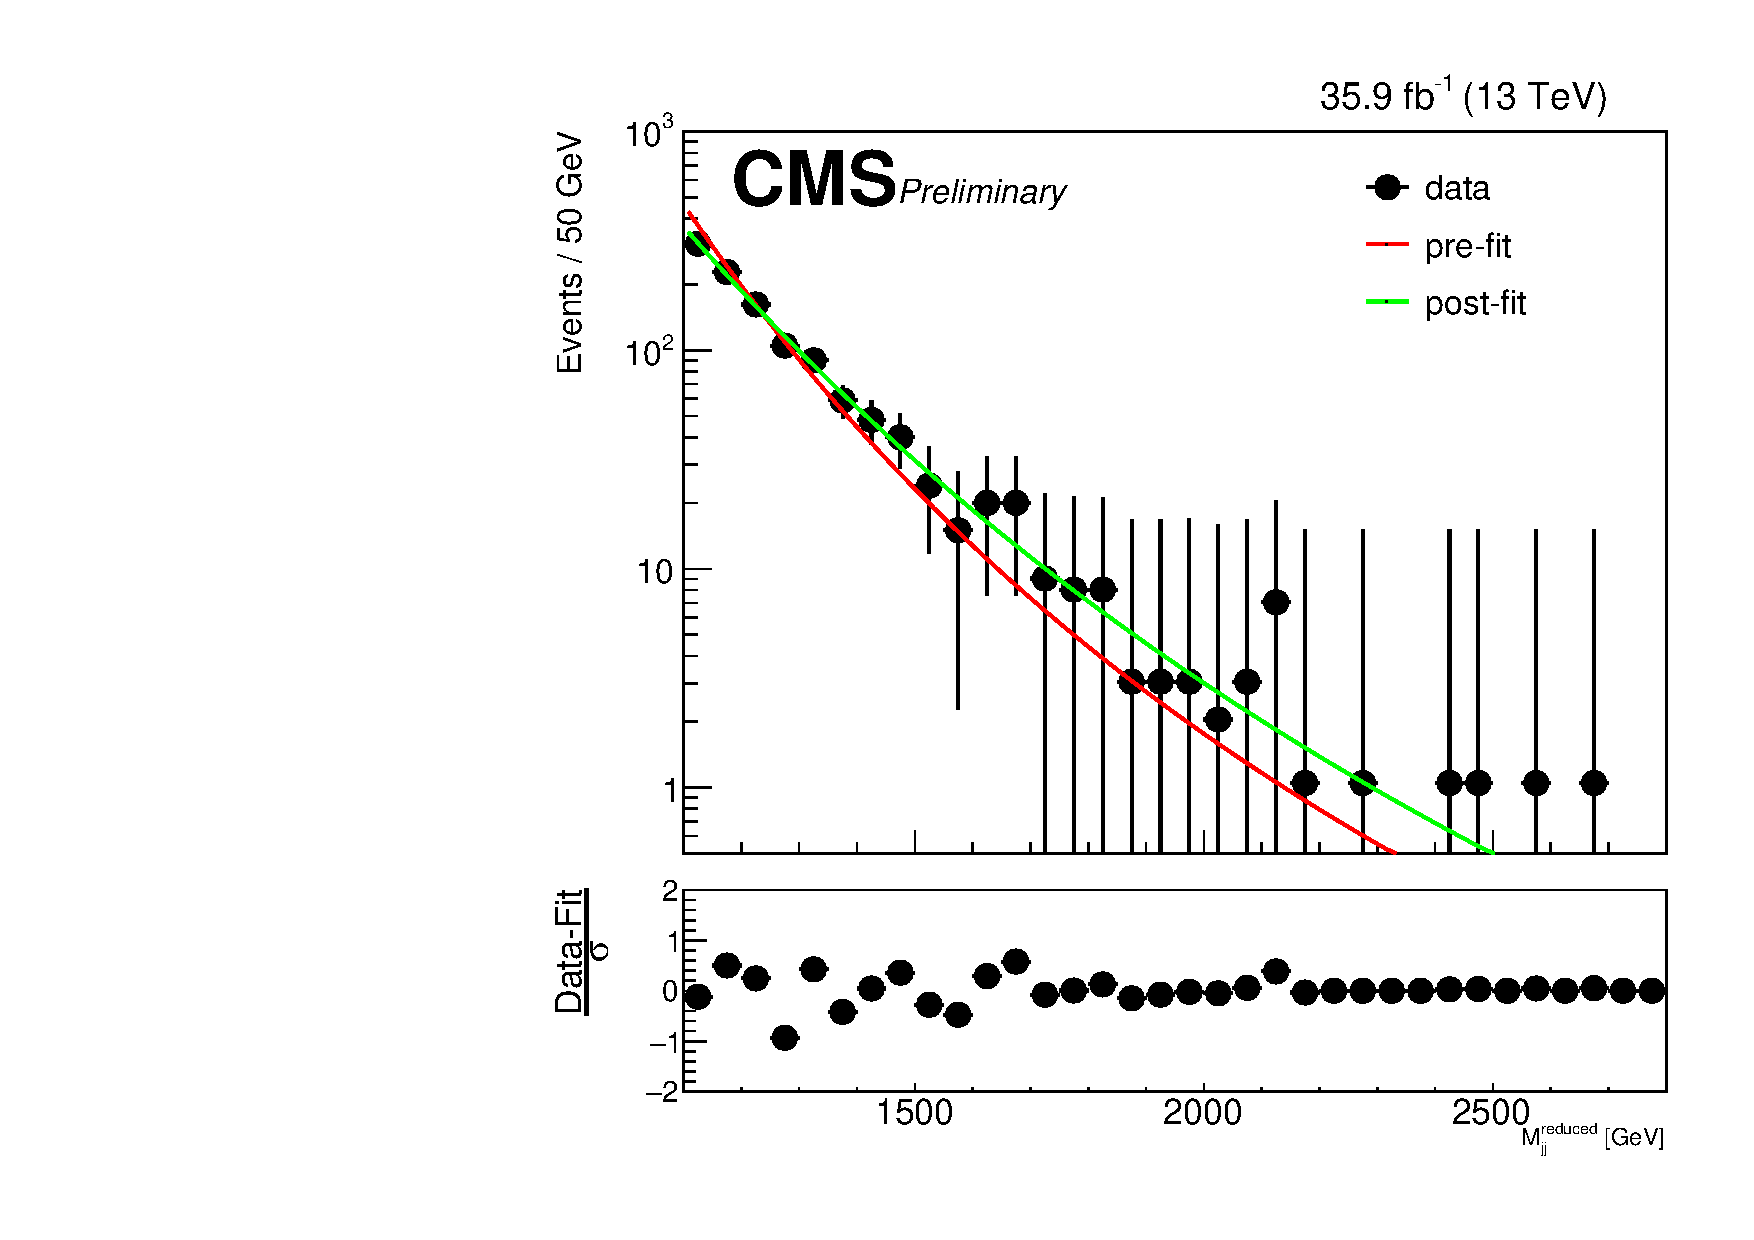
\includegraphics[width=0.5\textwidth]{Figures/aa/anti_TT.pdf} &
   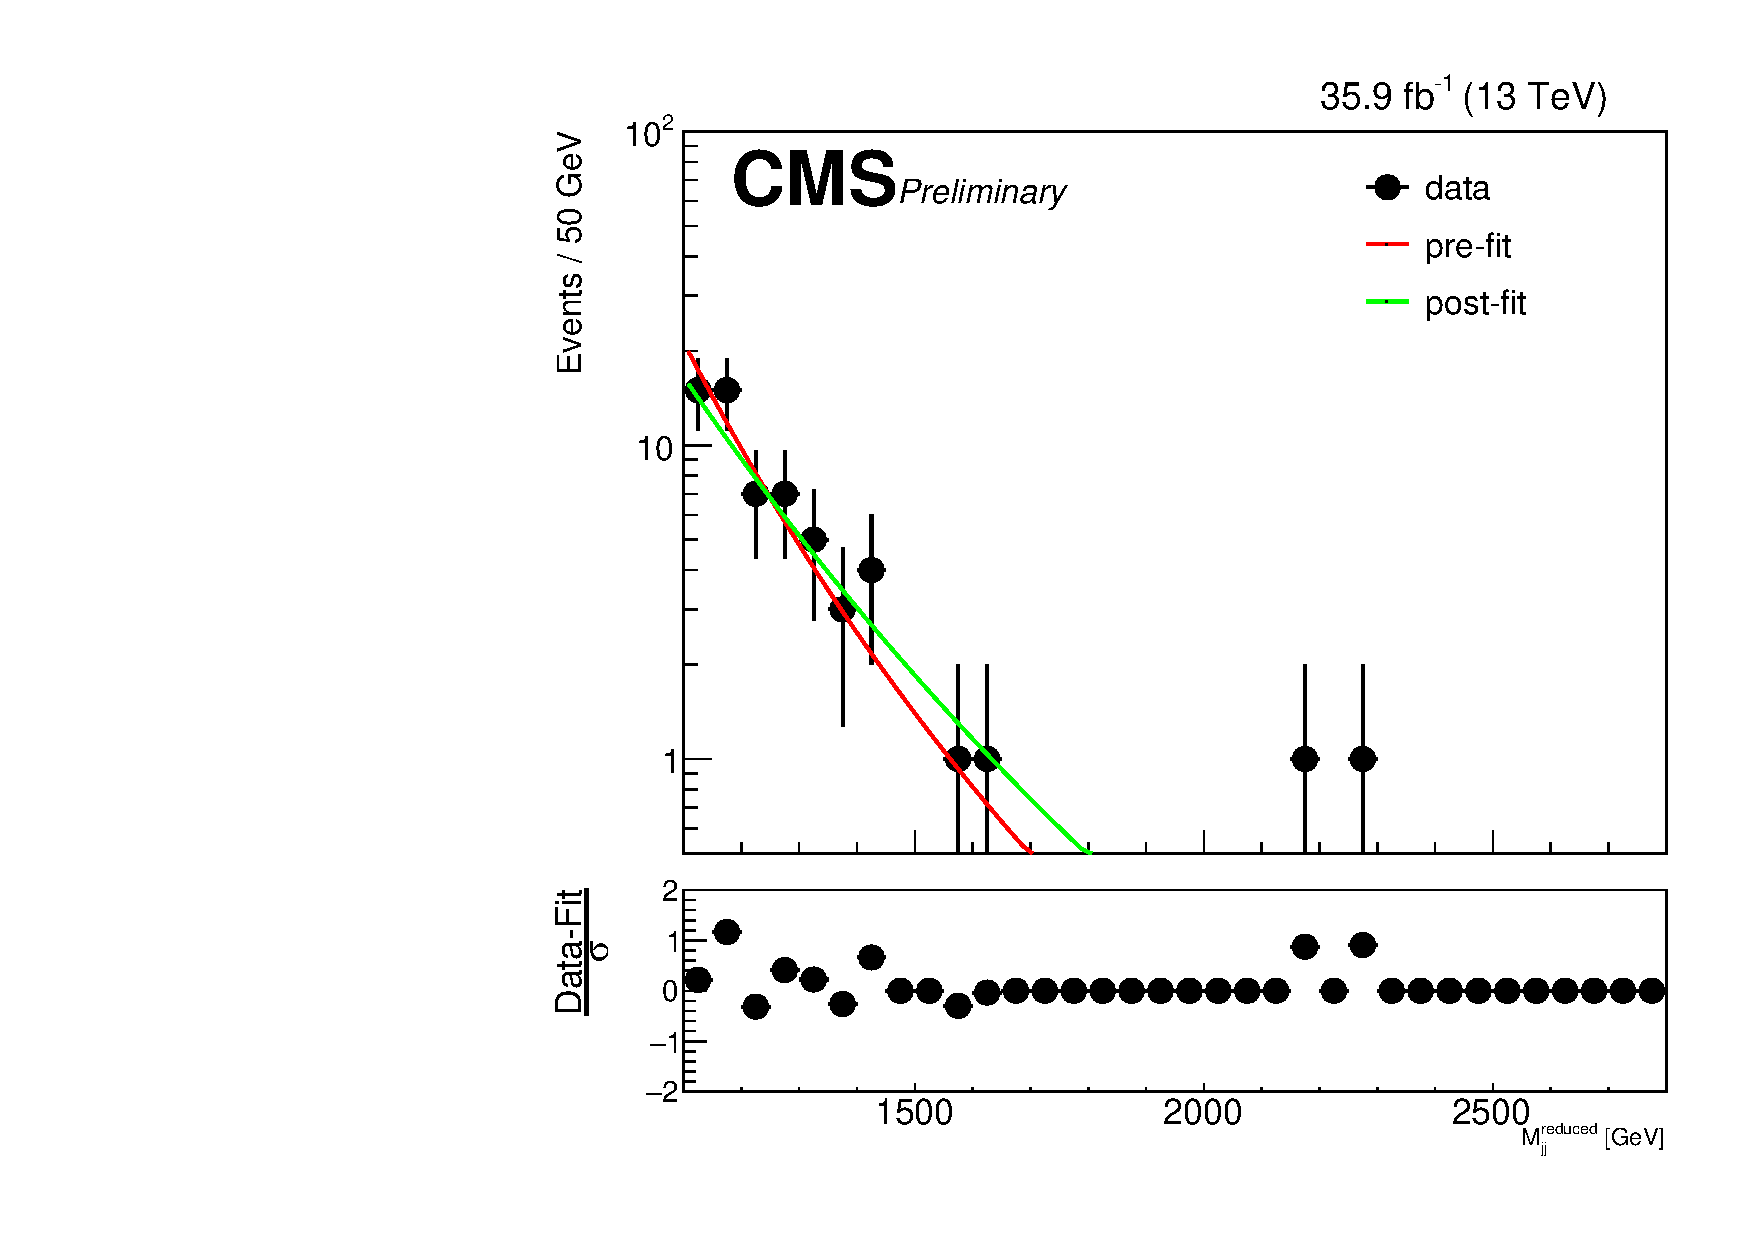
\includegraphics[width=0.5\textwidth]{Figures/aa/data_TT.pdf}
  \end{tabular}
  \caption{The pre-fit and post-fit on the data in anti-tag region (left) and signal region (right) in LL category (top) and TT category (buttom).}
  \label{fig:hvt_brs}
\end{figure}

\end{itemize}